\documentclass[margin=1pt]{standalone}
\usepackage{color,xcolor}
\usepackage{makecell}
\usepackage{tikz-qtree, tikz}
\usetikzlibrary{arrows.meta,bending}
\usetikzlibrary{calc,trees,positioning,arrows,chains,shapes, shapes.geometric,%
    decorations.pathreplacing,decorations.pathmorphing,decorations.markings,shapes,%
    matrix,shapes.symbols,positioning,angles,quotes,patterns}
\usepackage[utf8]{inputenc}

\def\centerarc[#1](#2)(#3:#4:#5)% Syntax: [draw options] (center) (initial angle:final angle:radius)
    { \draw[#1] ($(#2)+({#5*cos(#3)},{#5*sin(#3)})$) arc (#3:#4:#5); }

%See https://tex.stackexchange.com/a/29367/1952
\makeatletter
\tikzset{% customization of pattern
        hatch distance/.store in=\hatchdistance,
        hatch distance=5pt,
        hatch thickness/.store in=\hatchthickness,
        hatch thickness=5pt
        }
\pgfdeclarepatternformonly[\hatchdistance,\hatchthickness]{north east hatch}% name
    {\pgfqpoint{-1pt}{-1pt}}% below left
    {\pgfqpoint{\hatchdistance}{\hatchdistance}}% above right
    {\pgfpoint{\hatchdistance-1pt}{\hatchdistance-1pt}}%
    {
        \pgfsetcolor{\tikz@pattern@color}
        \pgfsetlinewidth{\hatchthickness}
        \pgfpathmoveto{\pgfqpoint{0pt}{0pt}}
        \pgfpathlineto{\pgfqpoint{\hatchdistance}{\hatchdistance}}
        \pgfusepath{stroke}
    }
\makeatother

% Drawing spirals
\makeatletter
\newif\ifspiral@is@clockwise
  \pgfkeys{
    spiral/.is family,
    spiral,
    start angle/.initial=0,
    end angle/.initial=0,
    start radius/.initial=0,
    end radius/.initial=1,
    revolutions/.initial=2,
    name/.initial=,
    center/.initial={(0,0)},
    sample rate/.initial =5,
    clockwise spiral/.is if=spiral@is@clockwise,
    clockwise spiral/.default=false,
    clockwise/.style={clockwise spiral=true},
    default spiral/.style={start angle=0,end angle=0, start radius=0, end radius=1, revolutions=2, name=, center={(0,0)}, sample rate=5, clockwise spiral=false}
  }
  \newcommand\spiral[2][]{
    \pgfkeys{spiral, default spiral,#2,
      start angle/.get=\spiral@start@angle,
      end angle/.get=\spiral@end@angle,
      start radius/.get=\spiral@start@radius,
      end radius/.get=\spiral@end@radius,
      revolutions/.get=\spiral@revolutions,
      name/.get=\spiral@name,
      sample rate/.get=\spiral@sample@rate,
      center/.get=\spiral@center
      }
  \def\spiral@start@name{}
  \def\spiral@end@name{}
  \ifspiral@is@clockwise
        \renewcommand*{\spiral@start@angle}{\pgfkeysvalueof{/spiral/end angle}}
        \renewcommand*{\spiral@end@angle}{\pgfkeysvalueof{/spiral/start angle}}
        \renewcommand*{\spiral@start@radius}{\pgfkeysvalueof{/spiral/end radius}}
        \renewcommand*{\spiral@end@radius}{\pgfkeysvalueof{/spiral/start radius}}
        \if\relax\detokenize{\spiral@name}\relax
        \else
          \renewcommand*{\spiral@start@name}{\spiral@name end}
          \renewcommand*{\spiral@end@name}{\spiral@name start}
        \fi
    \else
        \if\relax\detokenize{\spiral@name}\relax
        \else
          \renewcommand*{\spiral@start@name}{\spiral@name start}
          \renewcommand*{\spiral@end@name}{\spiral@name end}
        \fi
  \fi
  \pgfmathsetmacro{\spiral@domain}{\spiral@end@angle+\spiral@revolutions*360}
  \pgfmathsetmacro{\spiral@growth}{180*(\spiral@end@radius-\spiral@start@radius)/(pi*(\spiral@domain-\spiral@start@angle))}
  \draw [#1,
         shift={\spiral@center},
         domain=\spiral@start@angle*pi/180:\spiral@domain*pi/180,
         variable=\t,
         smooth,
         samples=int(\spiral@domain/\spiral@sample@rate)] node[coordinate,shift={(\spiral@start@angle:\spiral@start@radius)}](\spiral@start@name){} plot ({\t r}: {\spiral@start@radius+\spiral@growth*\t-\spiral@growth*\spiral@start@angle*pi/180}) node[coordinate](\spiral@end@name){}
  }
\makeatother

\definecolor{myblue}{HTML}{0072BD}
\definecolor{mygreen}{HTML}{258F1B}
\definecolor{myred}{HTML}{C4000C}

\newcommand{\Ms}{\ensuremath{M_\mathrm{s}}} % Martensite start Temperature
\newcommand{\Mf}{\ensuremath{M_\mathrm{f}}} % Martensite finish Temperature
\newcommand{\As}{\ensuremath{A_\mathrm{s}}} % Austenite start Temperature
\newcommand{\Af}{\ensuremath{A_\mathrm{f}}} % Austenite finish Temperature

% \usetikzlibrary{decorations.pathreplacing,arrows,shapes,positioning,shadows,calc}
% \usetikzlibrary{decorations, decorations.text,backgrounds}
% \tikzset{every picture/.style={font issue=\footnotesize},
%     font issue/.style={execute at begin picture={#1\selectfont}}
% }

\tikzset{
  pivot/.pic = {
    % screen (with border)
    \node (piv) {};
    % \centerarc[thick](piv.center) (45:315:0.4)
    \spiral[thick]{start radius=0.01, end radius=0.25, revolutions=3, center={(piv.center)}, clockwise, name=clockwisespiral};
    \draw [black,thick,domain=25:335] plot ({0.35*cos(\x)}, {0.35*sin(\x)});
    \draw[thick] ($(piv.center)+({0.35*cos(25)},{0.35*sin(25)})$) -- +(0.5cm,0) node (end1){};
    \draw[thick] ($(piv.center)+({0.35*cos(25)},{-0.35*sin(25)})$) -- +(0.5cm,0) node (end2){};
    \draw[thick] (end1.center) -- (end2.center);
    % \node(-m) [comp, pic actions, monitor]
    %   {\phantom{\parbox{\linewidth}{\tikzpictext}}};
    % % display (without border)
    % \node[comp, pic actions, display] {\tikzpictext};
    % \begin{scope}[x = (-m.east), y = (-m.north)]
    %   % filling the lower part
    %   \path[pic actions, draw = none]
    %     ([yshift=2\pgflinewidth]-0.1,-1) -- (-0.1,-1.3) -- (-1,-1.3) --
    %     (-1,-2.4) -- (1,-2.4) -- (1,-1.3) -- (0.1,-1.3) --
    %     ([yshift=2\pgflinewidth]0.1,-1);
    %   % filling the border of the lower part
    %   \path[ut]
    %     (-1,-2.4) rectangle (1,-1.3)
    %     (-0.9,-1.4) -- (-0.7,-2.3) -- (0.7,-2.3) -- (0.9,-1.4) -- cycle;
    %   % drawing the frame of the whole computer
    %   \path[pic actions, fill = none]
    %     (-1,1) -- (-1,-1) -- (-0.1,-1) -- (-0.1,-1.3) -- (-1,-1.3) --
    %     (-1,-2.4) coordinate(sw)coordinate[pos=0.5] (-b west) --
    %     (1,-2.4) -- (1,-1.3) coordinate[pos=0.5] (-b east) --
    %     (0.1,-1.3) -- (0.1,-1) -- (1,-1) -- (1,1) -- cycle;
    %   % node around the whole computer
    %   \node(-c) [fit = (sw)(-m.north east), inner sep = 0pt] {};
    % \end{scope}
  }
}


\begin{document}
\begin{tikzpicture}
% \begin{tikzpicture}[every node/.style={draw, outer sep=0pt,ultra thick,font=\footnotesize}]

% \tikzstyle{damper}=[thick,decoration={markings,
%   mark connection node=dmp,
%   mark=at position 0.1 with
%   {
%     \node (dmp) [thick,circle, inner sep=0pt,transform shape,rotate=-90,minimum width=15pt,minimum height=3pt] {};
%     \spiral[thick]{start radius=0.01, end radius=0.25, revolutions=3, center={(M.center)}, clockwise, name=clockwisespiral};
%     % \node (dmp) [thick,circle, inner sep=0pt,transform shape,rotate=-90,minimum width=15pt,minimum height=3pt,draw=none] {};
%     % \draw [thick] ($(dmp.north east)+(2pt,0)$) -- (dmp.south east) -- (dmp.south west) -- ($(dmp.north west)+(2pt,0)$);
%     % \draw [thick] ($(dmp.north)+(0,-5pt)$) -- ($(dmp.north)+(0,5pt)$);
%   }
% }, decorate]

% \tikzstyle{pivot}=[draw, circle,fill = white, outer sep=0pt,ultra thick,font=\footnotesize]
% \tikzstyle{pivot}=[draw,decoration={
%     \node[draw, circle] (piv) {};
%     % \spiral[thick]{start radius=0.01, end radius=0.25, revolutions=3, center={(piv.center)}, clockwise, name=clockwisespiral};
%     }]
\tikzstyle{sma}=[ultra thick,decorate,decoration={zigzag,pre length=4mm,post length=4mm,segment length=5mm, amplitude=2.5mm}]
\tikzstyle{spring}=[ultra thick,decoration={aspect=0.5,pre length=4mm,post length=4mm,segment length=4mm, amplitude=2.5mm,coil},decorate]
\tikzstyle{ground}=[pattern=north east hatch, hatch distance=2.5mm, hatch thickness=1pt, fill,draw=none,minimum width=2mm,minimum height=0.1mm]

\tikzstyle{smalong}=[ultra thick,decorate,decoration={zigzag,pre length=4mm,post length=4mm,segment length=9mm, amplitude=2.5mm}]
\tikzstyle{springshort}=[ultra thick,decoration={aspect=0.5,pre length=4mm,post length=4mm,segment length=2mm, amplitude=2.5mm,coil},decorate]

\tikzstyle{smarest}=[ultra thick,decorate,decoration={zigzag,pre length=4mm,post length=4mm,segment length=3.5mm, amplitude=2.5mm}]
\tikzstyle{springrest}=[ultra thick,decoration={aspect=0.5,pre length=4mm,post length=4mm,segment length=1.5mm, amplitude=2.5mm,coil},decorate]

% \tikzstyle{ground}=[fill,pattern=north east lines,draw=none,minimum width=2mm,minimum height=0.1mm]
% \tikzstyle{damper}=[thick,decoration={markings,
%   mark connection node=dmp,
%   mark=at position 0.5 with
%   {
%     \node (dmp) [thick,inner sep=0pt,transform shape,rotate=-90,minimum width=15pt,minimum height=3pt,draw=none] {};
%     \draw [thick] ($(dmp.north east)+(2pt,0)$) -- (dmp.south east) -- (dmp.south west) -- ($(dmp.north west)+(2pt,0)$);
%     \draw [thick] ($(dmp.north)+(0,-5pt)$) -- ($(dmp.north)+(0,5pt)$);
% }
%   }, decorate]
    % SMA - Spring (Hot)
    \node[inner sep=0pt] (piv1) at (0,0)
    {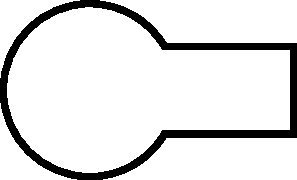
\includegraphics[scale=0.3]{pivot.pdf}};
    \node[inner sep=0pt] (slide1) at ($(piv1.center)+(-0.3,-0.62)$)
    {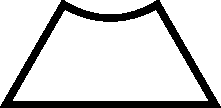
\includegraphics[scale=0.3]{slide.pdf}};
    \node (ground) [ground,anchor=north,minimum width=1cm,yshift=1] at (slide1.south) {};
    \spiral[thick]{start radius=0.01, end radius=0.35, revolutions=3, center={($(piv1.center)-(0.3,0)$)}, clockwise, name=clockwisespiral};

    \node[inner sep=0pt,rotate=180] (piv2) at (10,0)
    {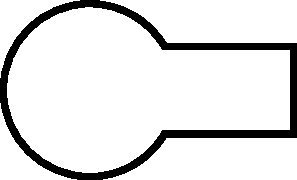
\includegraphics[scale=0.3]{pivot.pdf}};
    \node[inner sep=0pt] (slide2) at ($(piv2.center)+(0.3,-0.62)$)
    {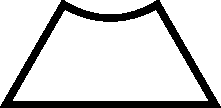
\includegraphics[scale=0.3]{slide.pdf}};
    \node (ground2) [ground,anchor=north,minimum width=1cm,yshift=-5] at (slide2.south) {};
    \draw[draw,thick] ($(slide2.south)+(0.3,-0.08)$) circle (2.5pt);
    \draw[draw,thick] ($(slide2.south)+(-0.3,-0.08)$) circle (2.5pt);
    \draw[draw,thick, anchor=center,radius=2,yshift=-5] (ground2.north east) -- (ground2.north west);
    \spiral[thick]{start radius=0.01, end radius=0.35, revolutions=3, center={($(piv2.center)-(-0.3,0)$)}, clockwise, name=clockwisespiral};

    \draw[draw,ultra thick] ($(piv1.center)+(0.71,0)$) node(beamend1){} -- ($(piv2.center)+(-0.71,0)$) node(beamend2){};
    \node[yshift=1.5cm, draw=none] (xl) at (beamend1.center) {};
    \node[yshift=1.5cm, draw=none] (xr) at (beamend2.center) {};
    \draw[|-|] (xl.center)-- node[above, draw=none] {$L$} (xr.center);
    \draw[latex-latex] (xl.center)-- (xr.center);



    % \pic(comp)[draw,rotate=30] {pivot} node (M) {};
    % \draw [thick] ($(M.center)+({-0.55*sin(25)},{-0.55*sin(25)})$) -- +(-0.3,-0.5) node (end1){};
    % \draw [thick] ($(M.center)+({0.55*sin(25)},{-0.55*sin(25)})$) -- +(0.3,-0.5) node (end2){};
    %     \draw[thick] (end1.center) -- (end2.center);
    %  \draw [ultra thick] (M.east) -- +(2cm,0cm) pic {pivot};


    %
    % % \node[pivot] (M) [minimum width=20,minimum height=20] {};
    % % \spiral[thick]{start radius=0.01, end radius=0.25, revolutions=3, center={(M.center)}, clockwise, name=clockwisespiral};
    % \node (ground) [ground,anchor=north,yshift=-0.25cm,minimum width=1cm] at (M.south) {};
    % \draw[ultra thick] (ground.north east) -- (ground.north west);
    % \draw [ultra thick] (M.south west) ++ (0.2cm,-0.125cm) circle (0.1cm)  (M.south east) ++ (-0.2cm,-0.125cm) circle (0.1cm);
    % \node (groundL) at (M.east) [ground, xshift=-4cm, rotate=-90, minimum height=0.1mm, minimum width=8mm] {};
    % \draw[ultra thick] (groundL.north west) -- (groundL.north east);
    % \node (groundR) at (M.west) [ground, xshift=+6cm, rotate=90, minimum height=0.1mm, minimum width=8mm] {};
    % \draw[ultra thick] (groundR.north west) -- (groundR.north east);
    % \draw[spring, color=mygreen] (M.east) -- node[draw=none, anchor=south, yshift=+4mm] {Bias-Spring} (groundR.north);
    % \draw[sma, color=myred] (M.west) -- node[draw=none, anchor=south, yshift=+4mm] {Hot SMA} (groundL.north);
    %
    %
    % % Cold SMA Bias Spring
    % \begin{scope}[yshift=3cm]
    %     \node (Mc) [minimum width=20,minimum height=20] at (2,0){};
    %     \node (ground) [ground,anchor=north,yshift=-0.25cm,minimum width=1cm] at (Mc.south) {};
    %     \draw[ultra thick] (ground.north east) -- (ground.north west);
    %     \draw [ultra thick] (Mc.south west) ++ (0.2cm,-0.125cm) circle (0.1cm)  (Mc.south east) ++ (-0.2cm,-0.125cm) circle (0.1cm);
    %
    %     \node (groundL) at (Mc.east) [ground, xshift=-6cm, rotate=-90, minimum height=0.1mm, minimum width=8mm] {};
    %     \draw[ultra thick] (groundL.north west) -- (groundL.north east);
    %     \node (groundR) at (Mc.west) [ground, xshift=+4cm, rotate=90, minimum height=0.1mm, minimum width=8mm] {};
    %     \draw[ultra thick] (groundR.north west) -- (groundR.north east);
    %
    %     \draw[springshort, color=mygreen] (Mc.east) -- node[draw=none, anchor=south, yshift=+4mm] {Bias-Spring} (groundR.north);
    %     \draw[smalong, color=myblue] (Mc.west) -- node[draw=none, anchor=south, yshift=+4mm] {Cold SMA} (groundL.north);
    % \end{scope}
    %
    % \node[yshift=+1.5cm, draw=none] (xc) at (M.south) {};
    % \node[yshift=-1.5cm, draw=none] (xh) at (Mc.south) {};
    % \draw[|-|] (xc.center)-- node[above, draw=none] {$\Delta x = x_1 - x_2$} (xh.center);
    % \draw[latex-latex] (xc.center)-- (xh.center);
    % \draw[dotted] (M.center)--(xc.center);
    % \draw[dotted] (Mc.center)--(xh.center);
    %
    % % Disconnected SMA Bias Spring
    % \begin{scope}[yshift=6cm]
    %     \node (Mr) [minimum width=20,minimum height=20] at (2.5,0){};
    %     \node (groundRR) [ground,anchor=north,yshift=-0.25cm,minimum width=1cm] at (Mr.south) {};
    %     \draw[ultra thick] (groundRR.north east) -- (groundRR.north west);
    %     \draw [ultra thick] (Mr.south west) ++ (0.2cm,-0.125cm) circle (0.1cm)  (Mr.south east) ++ (-0.2cm,-0.125cm) circle (0.1cm);
    %
    %     \node (groundLR) at (Mr.east) [ground, xshift=-6.5cm, rotate=-90, minimum height=0.1mm, minimum width=8mm] {};
    %     \draw[ultra thick] (groundLR.north west) -- (groundLR.north east);
    %     \node (groundRR) at (Mr.west) [ground, xshift=+3.5cm, rotate=90, minimum height=0.1mm, minimum width=8mm] {};
    %     \draw[ultra thick] (groundRR.north west) -- (groundRR.north east);
    %
    %     \draw[springrest, color=mygreen] (Mr.east) -- node[draw=none, anchor=south, yshift=+4mm] {Bias-Spring $(K_\mathrm{BS})$} (groundRR.north);
    %     \draw[smarest, color=black] ($(Mr.west)-(3.25,0)$) -- node[draw=none, anchor=south, yshift=+4mm] {SMA} (groundLR.north);
    % \end{scope}
    %
    % % \node[yshift=-1.25cm, draw=none] (xcr) at (groundLR.north) {}; % Start of resting SMA
    % \node[yshift=-1.25cm, draw=none] (xcr) at ($(Mr.west)-(3.25,0)$) {};
    % \node[yshift=-1.25cm, draw=none] (xhr) at (Mr.center) {};
    % \draw[|-|] (xcr.center)-- node[below, draw=none] {$x_\mathrm{off}$} (xhr.center);
    % \draw[latex-latex] (xcr.center)-- (xhr.center);
    % % \draw[dotted] (groundLR.north)--(xcr.center); % Start of resting SMA
    % \draw[dotted] ($(Mr.west)-(3.25,0)$)--(xcr.center);
    % \draw[dotted] (Mr.center)--(xhr.center);
    %
    % \node[yshift=-0.75cm, draw=none] (xcr) at (groundLR.north) {};
    % \node[yshift=-0.75cm, draw=none] (xhr) at ($(Mr.west)-(3.25,0)$) {};
    % \draw[|-|] (xcr.center)-- node[below, draw=none] {$L_\mathrm{SMA}$} (xhr.center);
    % \draw[latex-latex] (xcr.center)-- (xhr.center);
    % \draw[dotted] (groundLR.north)--(xcr.center);
    % \draw[dotted] ($(Mr.west)-(3.25,0)$)--(xhr.center);

\end{tikzpicture}
\end{document}
